\documentclass[11pt]{article}

\usepackage{amssymb, amsmath, mathtools, color, fontspec}
\usepackage{ifxetex, ifluatex, microtype}

\setsansfont{Roboto}
\setmainfont{Roboto}

\usepackage[affil-it]{authblk}

\PassOptionsToPackage{hyphens}{url} % url is loaded by hyperref

\usepackage[unicode=true]{hyperref}

\PassOptionsToPackage{usenames, dvipsnames}{color} % color is loaded by hyperref

\hypersetup{
            pdftitle={Lineage},
            pdfkeywords={cancer, heterogeneity},
            pdfborder={0 0 0},
            breaklinks=true}
\urlstyle{same}  % don't use monospace font for urls

\usepackage[margin=1in, letterpaper]{geometry}

\usepackage[]{biblatex}
\addbibresource{./manuscript/references.bib}


\usepackage{longtable,booktabs}
\usepackage{graphicx,grffile}
\makeatletter
\def\maxwidth{\ifdim\Gin@nat@width>\linewidth\linewidth\else\Gin@nat@width\fi}
\def\maxheight{\ifdim\Gin@nat@height>\textheight\textheight\else\Gin@nat@height\fi}
\makeatother
% Scale images if necessary, so that they will not overflow the page
% margins by default, and it is still possible to overwrite the defaults
% using explicit options in \includegraphics[width, height, ...]{}
\setkeys{Gin}{width=\maxwidth,height=\maxheight,keepaspectratio}
\IfFileExists{parskip.sty}{%
\usepackage{parskip}
}{% else
\setlength{\parindent}{0pt}
\setlength{\parskip}{6pt plus 2pt minus 1pt}
}
\setlength{\emergencystretch}{3em}  % prevent overfull lines
\providecommand{\tightlist}{%
  \setlength{\itemsep}{0pt}\setlength{\parskip}{0pt}}
\setcounter{secnumdepth}{0}
% Redefines (sub)paragraphs to behave more like sections
\ifx\paragraph\undefined\else
\let\oldparagraph\paragraph
\renewcommand{\paragraph}[1]{\oldparagraph{#1}\mbox{}}
\fi
\ifx\subparagraph\undefined\else
\let\oldsubparagraph\subparagraph
\renewcommand{\subparagraph}[1]{\oldsubparagraph{#1}\mbox{}}
\fi

% set default figure placement to htbp
\makeatletter
\def\fps@figure{htbp}
\makeatother

% Defines absolute value paired delimiter "\abs{}"
\DeclarePairedDelimiter\abs{\lvert}{\rvert}

\title{Lineage}

\author[a]{Adam Weiner}
\author[a]{Ali Farhat}
\author[a,b]{Aaron S. Meyer}

\affil[a]{Department of Bioengineering, Jonsson Comprehensive Cancer Center, Eli
and Edythe Broad Center of Regenerative Medicine and Stem Cell Research;
University of California, Los Angeles}
\affil[b]{Contact info}

\date{}

\newcommand{\beginsupplement}{\cleardoublepage%
      \setcounter{table}{0}
      \renewcommand{\thetable}{S\arabic{table}}%
      \setcounter{figure}{0}
      \renewcommand{\thefigure}{S\arabic{figure}}%
}

\begin{document}
\maketitle


\begin{abstract}
This is the abstract.
\end{abstract}


\hypertarget{summary-points}{%
\section{Summary points}\label{summary-points}}

\begin{itemize}
\tightlist
\item
  One
\item
  Two
\item
  Three
\end{itemize}

\hypertarget{introduction}{%
\section{Introduction}\label{introduction}}

This is the introduction.

\hypertarget{acknowledgements}{%
\section{Acknowledgements}\label{acknowledgements}}

This work was supported by NIH DP5-OD019815 to A.S.M. \textbf{Competing
financial interests:} The authors declare no competing financial
interests.

\hypertarget{author-contributions-statement}{%
\section{Author contributions
statement}\label{author-contributions-statement}}

A.S.M. conceived of the study. A.F., A.S.M, and A.W. performed the
computational analysis. All authors helped to design experiments and/or
analyze the data.

\beginsupplement

\hypertarget{supplement}{%
\section{Supplement}\label{supplement}}

\begin{figure}
\hypertarget{fig:supp1}{%
\centering
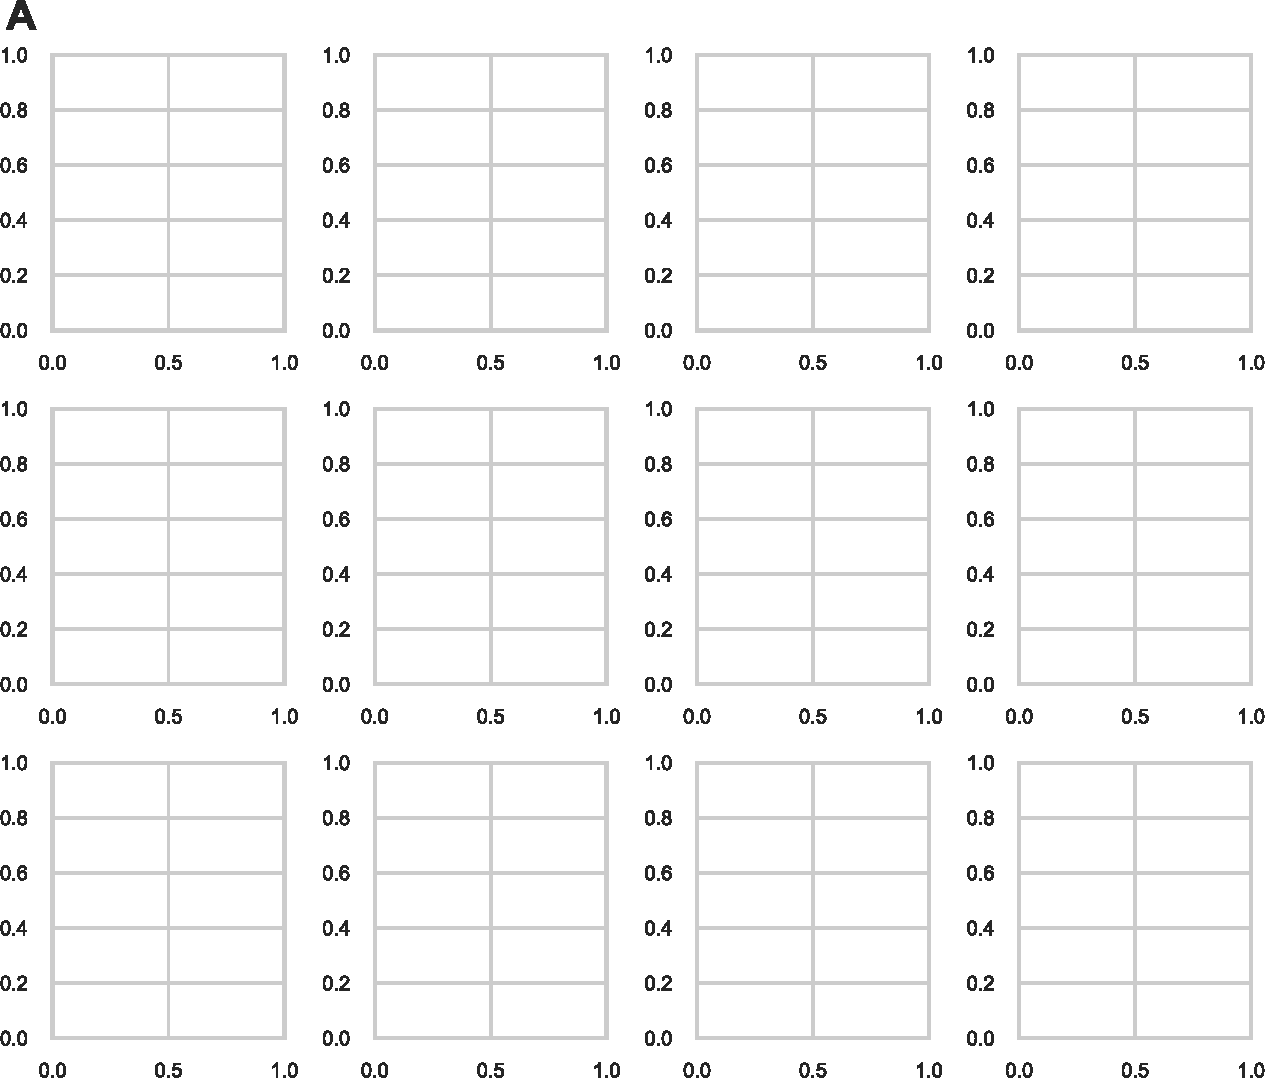
\includegraphics{./figures/figureS1.pdf}
\caption{\textbf{Title of supplement 1.} XXX}\label{fig:supp1}
}
\end{figure}

\begin{figure}
\hypertarget{fig:supp2}{%
\centering
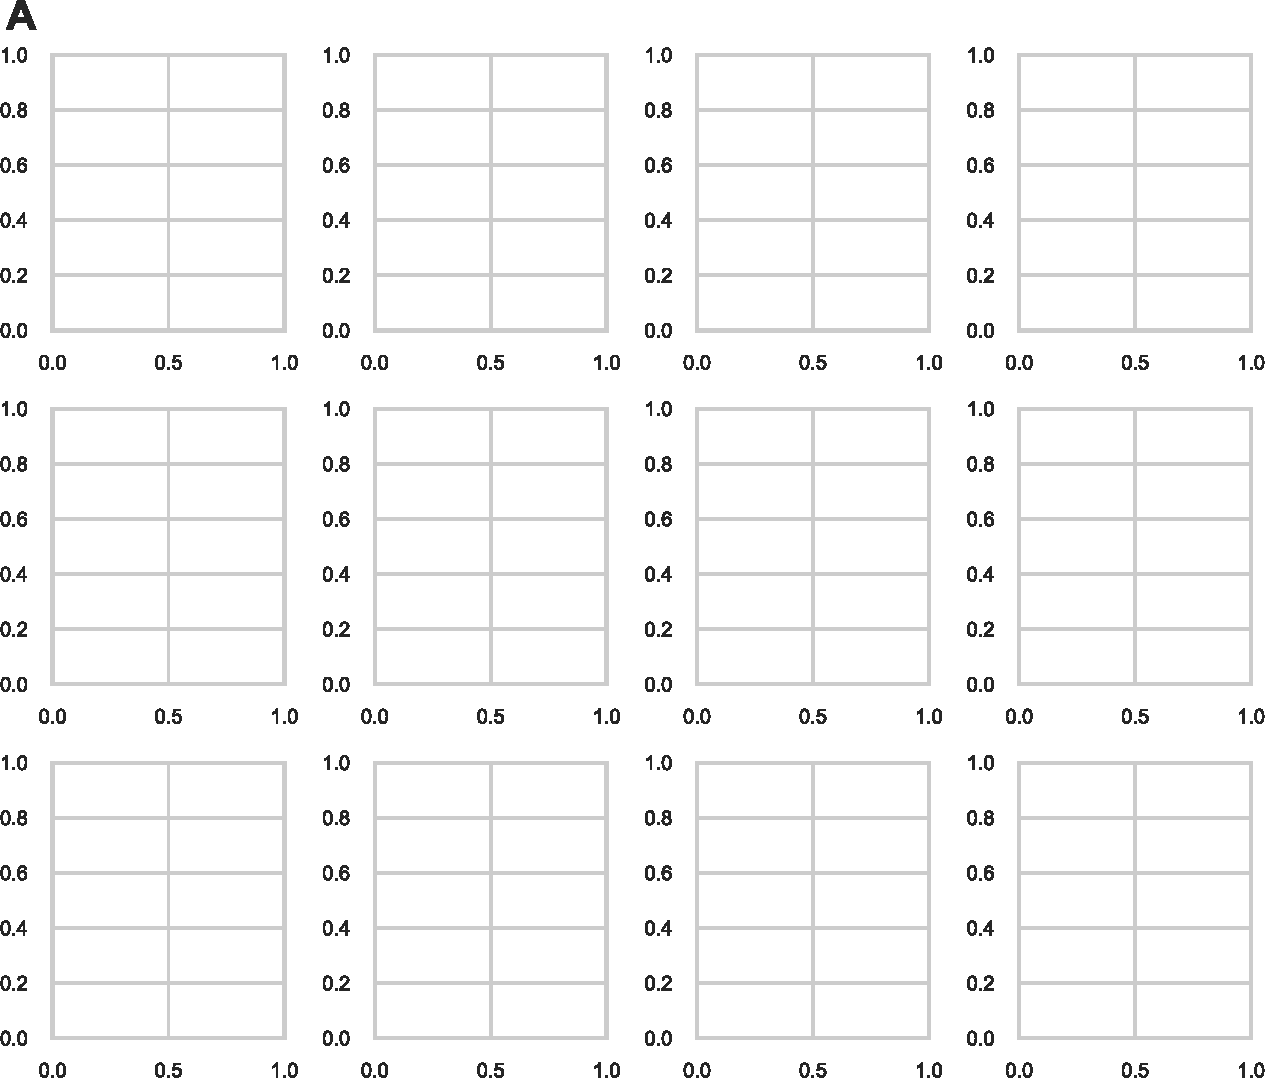
\includegraphics{./figures/figureS2.pdf}
\caption{\textbf{Title of supplement 2.} XXX}\label{fig:supp2}
}
\end{figure}

\begin{figure}
\hypertarget{fig:supp3}{%
\centering
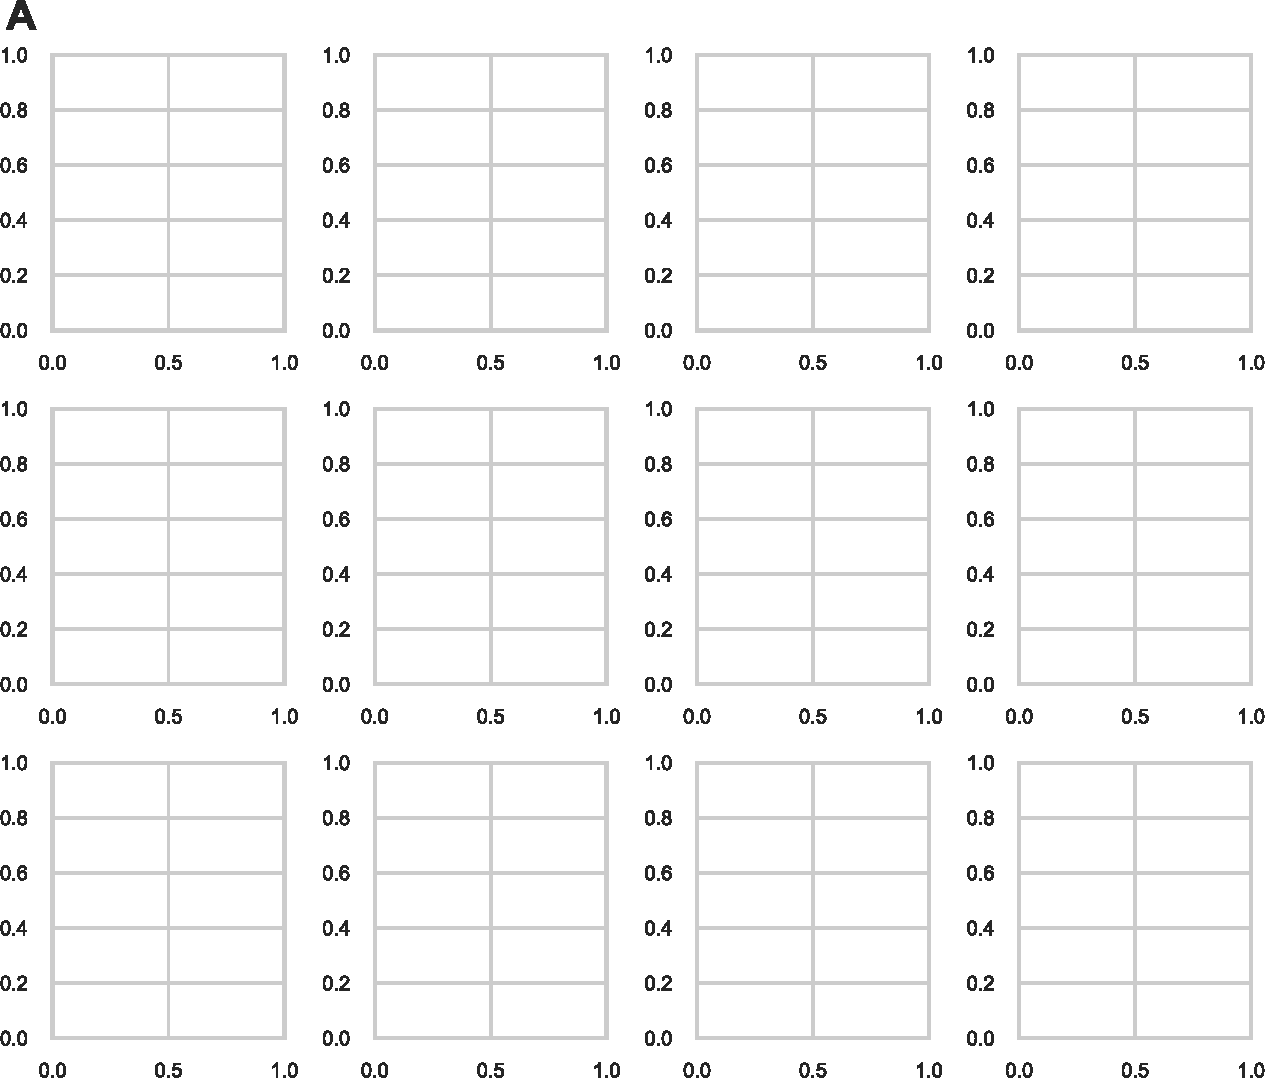
\includegraphics{./figures/figureS3.pdf}
\caption{\textbf{Title of supplement 3.} XXX}\label{fig:supp3}
}
\end{figure}

\begin{figure}
\hypertarget{fig:supp4}{%
\centering
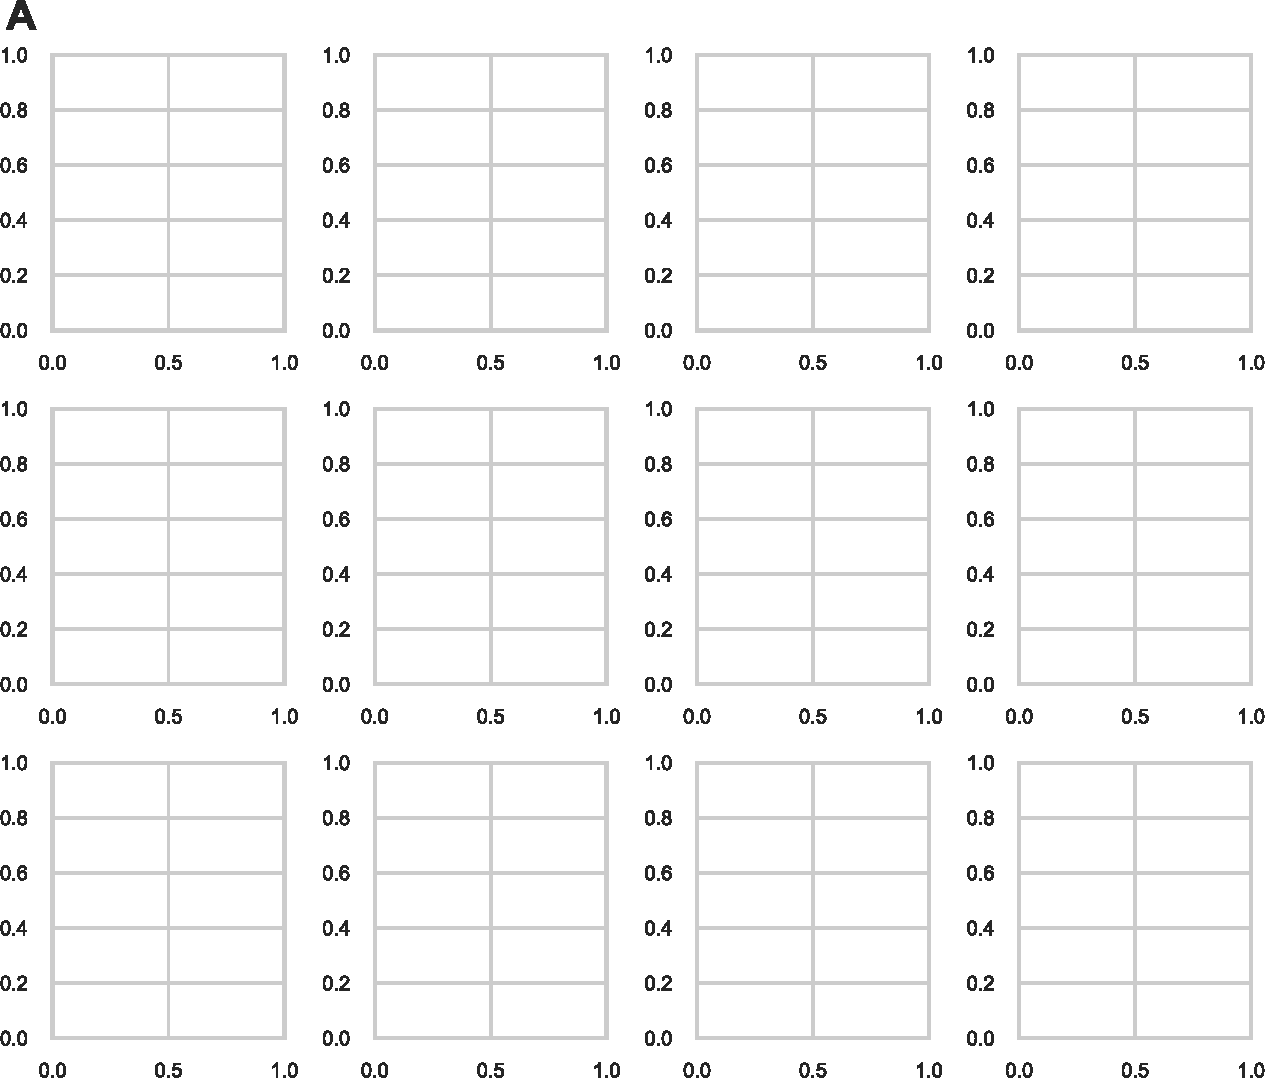
\includegraphics{./figures/figureS4.pdf}
\caption{\textbf{Title of supplement 4.} XXX}\label{fig:supp4}
}
\end{figure}

\begin{figure}
\hypertarget{fig:supp5}{%
\centering
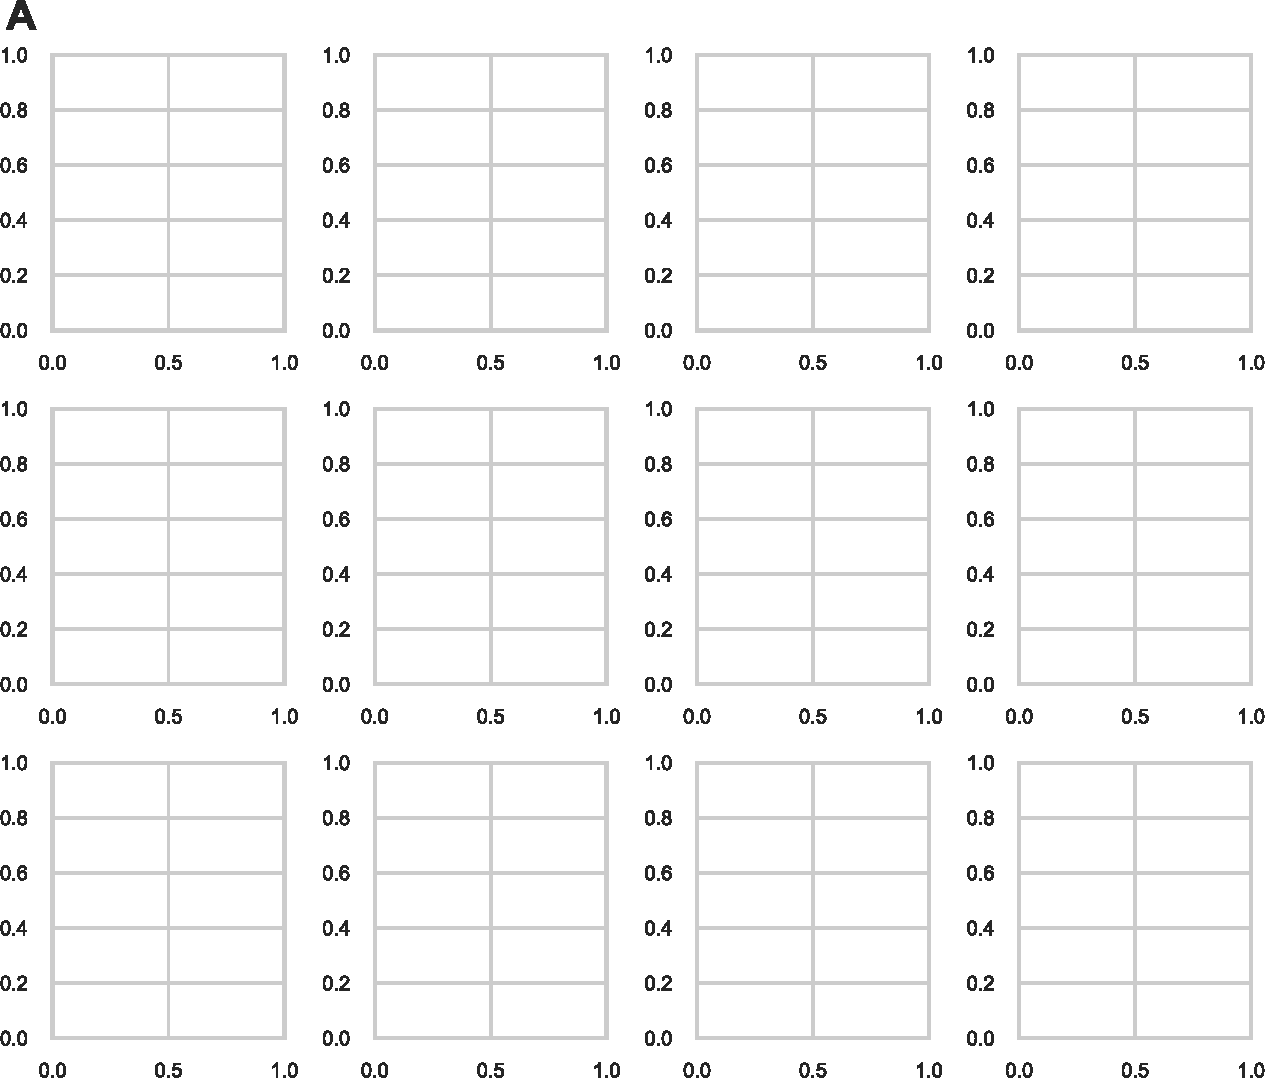
\includegraphics{./figures/figureS5.pdf}
\caption{\textbf{Title of supplement 5.} XXX}\label{fig:supp5}
}
\end{figure}

\cleardoublepage

\hypertarget{references}{%
\section{References}\label{references}}

\printbibliography

\end{document}